% move all configuration stuff into one file so we can focus on the content
\documentclass[aspectratio=169,hyperref={pdfpagelabels=false,colorlinks=true,linkcolor=white,urlcolor=lightblue},xcolor={table},t]{beamer}

%%%%%%%%%%%%%%%%%%%%%%%%%%%%%%%%%%%%%%%%%%%%%%%%%%%%%%%%%%%%%%%%%%%%%%%%%%%%%%%%%%
%%%%%%%%%%%%%%%%%%%%%%%%%%%%%%%%%%%%%%%%%%%%%%%%%%%%%%%%%%%%%%%%%%%%%%%%%%%%%%%%%%
% packages
\usepackage{pict2e}
\usepackage{epic}
\usepackage{amsmath,amsfonts,amssymb}
\usepackage{units}
\usepackage{fancybox}
\usepackage[absolute,overlay]{textpos} 
%\usepackage[table]{xcolor}
\usepackage{animate}
\usepackage{gensymb}
%\usepackage{graphicx}
%\usepackage{longtable}
\usepackage{multirow}
\usepackage{silence}
\usepackage{tikz}
\usepackage[backend=bibtex,style=ieee]{biblatex}
\AtEveryCitekey{\iffootnote{\tiny}{}}
%\addbibresource{include/references}



% fontsize
\let\Tiny=\tiny

%%%%%%%%%%%%%%%%%%%%%%%%%%%%%%%%%%%%%%%%%%%%%%%%%%%%%%%%%%%%%%%%%%%%%%%%%%%%%%%%%%
%%%%%%%%%%%%%%%%%%%%%%%%%%%%%%%%%%%%%%%%%%%%%%%%%%%%%%%%%%%%%%%%%%%%%%%%%%%%%%%%%%
% warnings
\pdfsuppresswarningpagegroup=1
\WarningFilter{biblatex}{Patching footnotes failed}
\WarningFilter{latexfont}{Font shape}
\WarningFilter{latexfont}{Some font shapes}
\WarningFilter{gensymb}{Not defining}


%%%%%%%%%%%%%%%%%%%%%%%%%%%%%%%%%%%%%%%%%%%%%%%%%%%%%%%%%%%%%%%%%%%%%%%%%%%%%%%%%%
%%%%%%%%%%%%%%%%%%%%%%%%%%%%%%%%%%%%%%%%%%%%%%%%%%%%%%%%%%%%%%%%%%%%%%%%%%%%%%%%%%
% theme & layout
\usetheme{Frankfurt}
\useinnertheme{rectangles}


%%%%%%%%%%%%%%%%%%%%%%%%%%%%%%%%%%%%%%%%%%%%%%%%%%%%%%%%%%%%%%%%%%%%%%%%%%%%%%%%%%
\setbeamertemplate{frametitle}[default][colsep=-4bp,rounded=false,shadow=false]
\setbeamertemplate{frametitle}
{%
    \nointerlineskip%
    %\vskip-0.5ex
    \begin{beamercolorbox}[wd=\paperwidth,ht=3.5ex,dp=0.6ex]{frametitle}
        \hspace*{1.3ex}\insertframetitle%
        
        \hspace*{1.3ex}\small\insertframesubtitle%
    \end{beamercolorbox}%
    \begin{textblock*}{100mm}(13.75cm,1cm)
        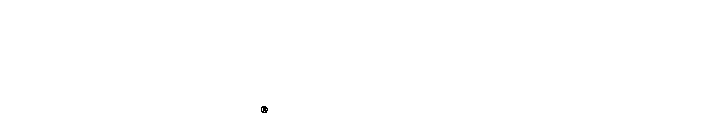
\includegraphics[height=.4cm,keepaspectratio]{../shared/Logo_GTCMT_white}
    \end{textblock*}
}


%%%%%%%%%%%%%%%%%%%%%%%%%%%%%%%%%%%%%%%%%%%%%%%%%%%%%%%%%%%%%%%%%%%%%%%%%%%%%%%%%%
\setbeamertemplate{title page}[default][colsep=-4bp,rounded=false,shadow=false]
\setbeamertemplate{title page}
{
    %\begin{textblock*}{100mm}(15cm,.51cm)
            %\href{https://github.com/alexanderlerch/ACA-Slides/blob/2nd_edition/\jobname.pdf}{\includegraphics[height=.5cm,keepaspectratio]{graph/Logo_github}}\hspace*{2ex}
    %\end{textblock*}
    %\begin{textblock*}{100mm}(15cm,1.3cm)
            %\href{\IEEELink}{\includegraphics[height=.5cm,keepaspectratio]{graph/icon/book}}\hspace*{2ex}
    %\end{textblock*}
    \vskip-10ex
    \begin{beamercolorbox}[wd=\paperwidth,ht=.7\paperheight,dp=0.6ex]{frametitle} %35ex
        %\begin{flushright}
            %\href{http://www.gtcmt.gatech.edu}{
\includegraphics[height=.8cm,keepaspectratio]{graph/Logo_GTCMT_black}}\hspace*{2ex}
        %\end{flushright}
        
        \hspace*{1.8ex}\LARGE\inserttitle%
        
        \vspace*{.5ex}
        
        \hspace*{1.3ex}\small\insertsubtitle%
        
        \vspace*{.5ex}
    \end{beamercolorbox}%
    \nointerlineskip%
    \begin{beamercolorbox}[wd=\paperwidth,ht=.4\paperheight,dp=0.6ex]{page number in head/foot}
        %\vspace*{-.5ex}
        \hspace*{1.7ex}\small\insertauthor%
        
        %\hspace*{1.7ex}\small }%
        
        \vspace*{12ex}
        \vfill
        \begin{flushright}
            \href{http://www.gtcmt.gatech.edu}{
\includegraphics[height=.5cm,keepaspectratio]{../shared/Logo_GTCMT_black}}\hspace*{2ex}
        \end{flushright}
    \end{beamercolorbox}%
}


%%%%%%%%%%%%%%%%%%%%%%%%%%%%%%%%%%%%%%%%%%%%%%%%%%%%%%%%%%%%%%%%%%%%%%%%%%%%%%%%%%
%\makeatother
\setbeamertemplate{footline}
{
  \leavevmode%
  \hbox{%
  \begin{beamercolorbox}[wd=.5\paperwidth,ht=2.25ex,dp=1ex,left,leftskip=1ex]{page number in head/foot}%
    \insertsubtitle
  \end{beamercolorbox}%
  \begin{beamercolorbox}[wd=.5\paperwidth,ht=2.25ex,dp=1ex,right,rightskip=1ex]{page number in head/foot}%
    \hfill
    \insertframenumber{} / \inserttotalframenumber
  \end{beamercolorbox}}%
  \vskip0pt%
}
%\makeatletter


%%%%%%%%%%%%%%%%%%%%%%%%%%%%%%%%%%%%%%%%%%%%%%%%%%%%%%%%%%%%%%%%%%%%%%%%%%%%%%%%%%
\beamertemplatenavigationsymbolsempty
\setbeamertemplate{navigation symbols}{}
\setbeamertemplate{blocks}[default]%[rounded=false,shadow=false]
\setbeamertemplate{itemize item}[square]
\setbeamertemplate{itemize subitem}[circle]
\setbeamertemplate{itemize subsubitem}[triangle]
\setbeamertemplate{enumerate item}[square]
\setbeamertemplate{enumerate subitem}[circle]
\setbeamertemplate{enumerate subsubitem}[circle]


%%%%%%%%%%%%%%%%%%%%%%%%%%%%%%%%%%%%%%%%%%%%%%%%%%%%%%%%%%%%%%%%%%%%%%%%%%%%%%%%%%
% colors
\setbeamercolor{structure}{fg=darkgray}
\setbeamercovered{transparent} %invisible
\setbeamercolor{bibliography entry author}{fg=black}
\setbeamercolor*{bibliography entry title}{fg=black}
\setbeamercolor*{bibliography entry note}{fg=black}
\setbeamercolor{frametitle}{fg=black}
\setbeamercolor{title}{fg=white}
\setbeamercolor{subtitle}{fg=white}
\setbeamercolor{frametitle}{fg=white}
\setbeamercolor{framesubtitle}{fg=white}
\setbeamercolor{mini frame}{fg=white, bg=black}
\setbeamercolor{section in head/foot}{fg=white, bg=darkgray}
\setbeamercolor{page number in head/foot}{fg=black, bg=gtgold}
\setbeamercolor{item projected}{fg=white, bg=black}

%---------------------------------------------------------------------------------

%%%%%%%%%%%%%%%%%%%%%%%%%%%%%%%%%%%%%%%%%%%%%%%%%%%%%%%%%%%%%%%%%%%%%%%%%%%%%%%%%%
%%%%%%%%%%%%%%%%%%%%%%%%%%%%%%%%%%%%%%%%%%%%%%%%%%%%%%%%%%%%%%%%%%%%%%%%%%%%%%%%%%
% title information
\title[]{MUSI6202: Digital Signal Processing for Music}   
\author[alexander lerch]{alexander lerch} 
%\institute{~}
%\date[Alexander Lerch]{}
%\titlegraphic{\vspace{-16mm}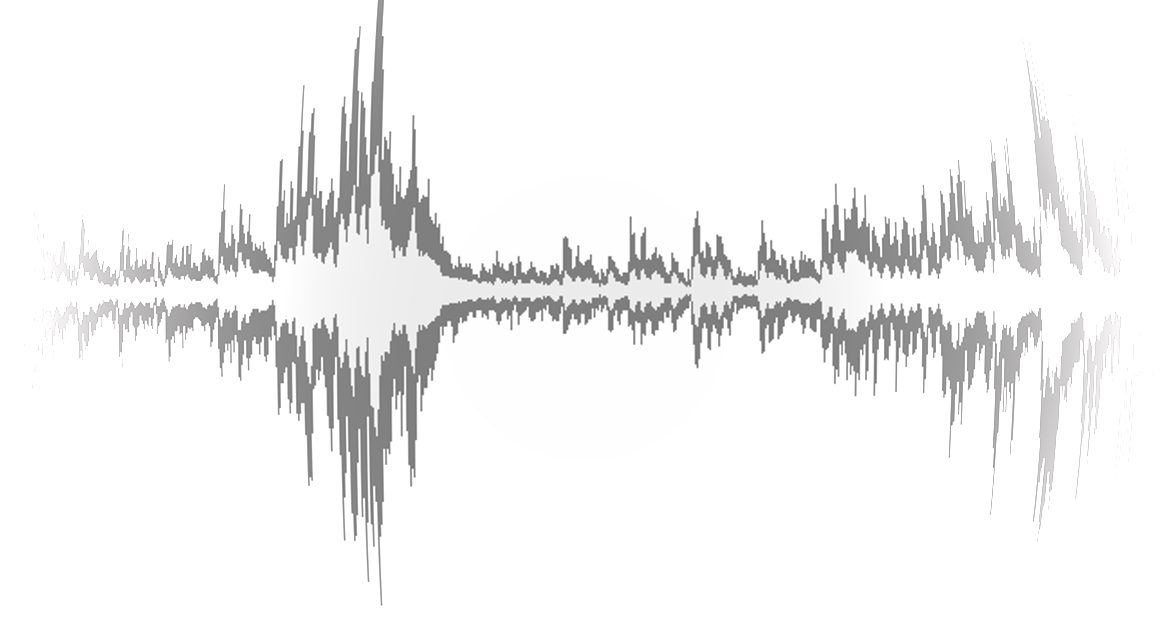
\includegraphics[width=\textwidth,height=3cm]{title}}

%%%%%%%%%%%%%%%%%%%%%%%%%%%%%%%%%%%%%%%%%%%%%%%%%%%%%%%%%%%%%%%%%%%%%%%%%%%%%%%%%%
%%%%%%%%%%%%%%%%%%%%%%%%%%%%%%%%%%%%%%%%%%%%%%%%%%%%%%%%%%%%%%%%%%%%%%%%%%%%%%%%%%
% colors
\definecolor{gtgold}{rgb}{.914, .664, 0} %0e7eed {rgb}{0.88,0.66,1,0.06} [234, 170, 0]/256 %96caff
\definecolor{darkgray}{rgb}{.15, .15, .15}
\definecolor{lightblue}{HTML}{0e7eed}
\definecolor{highlight}{rgb}{0, 0, 1} %_less!40

%%%%%%%%%%%%%%%%%%%%%%%%%%%%%%%%%%%%%%%%%%%%%%%%%%%%%%%%%%%%%%%%%%%%%%%%%%%%%%%%%%
%%%%%%%%%%%%%%%%%%%%%%%%%%%%%%%%%%%%%%%%%%%%%%%%%%%%%%%%%%%%%%%%%%%%%%%%%%%%%%%%%%
% relative paths
\graphicspath{{../graph/}}


%%%%%%%%%%%%%%%%%%%%%%%%%%%%%%%%%%%%%%%%%%%%%%%%%%%%%%%%%%%%%%%%%%%%%%%%%%%%%%%%%%
%%%%%%%%%%%%%%%%%%%%%%%%%%%%%%%%%%%%%%%%%%%%%%%%%%%%%%%%%%%%%%%%%%%%%%%%%%%%%%%%%%
% units
\setlength{\unitlength}{1mm}

%%%%%%%%%%%%%%%%%%%%%%%%%%%%%%%%%%%%%%%%%%%%%%%%%%%%%%%%%%%%%%%%%%%%%%%%%%%%%%%%%%
%%%%%%%%%%%%%%%%%%%%%%%%%%%%%%%%%%%%%%%%%%%%%%%%%%%%%%%%%%%%%%%%%%%%%%%%%%%%%%%%%%
% math
\DeclareMathOperator*{\argmax}{argmax}
\DeclareMathOperator*{\argmin}{argmin}
\DeclareMathOperator*{\atan}{atan}
\DeclareMathOperator*{\arcsinh}{arcsinh}
\DeclareMathOperator*{\sign}{sign}
\DeclareMathOperator*{\tcdf}{tcdf}
\DeclareMathOperator*{\si}{sinc}
\DeclareMathOperator*{\princarg}{princarg}
\DeclareMathOperator*{\arccosh}{arccosh}
\DeclareMathOperator*{\hwr}{HWR}
\DeclareMathOperator*{\flip}{flip}
\DeclareMathOperator*{\sinc}{sinc}
\DeclareMathOperator*{\floor}{floor}
\newcommand{\e}{{e}}
\newcommand{\jom}{\mathrm{j}\omega}
\newcommand{\jOm}{\mathrm{j}\Omega}
\newcommand   {\mat}[1]    		{\boldsymbol{\uppercase{#1}}}		%bold
\renewcommand {\vec}[1]    		{\boldsymbol{\lowercase{#1}}}		%bold

%%%%%%%%%%%%%%%%%%%%%%%%%%%%%%%%%%%%%%%%%%%%%%%%%%%%%%%%%%%%%%%%%%%%%%%%%%%%%%%%%%
%%%%%%%%%%%%%%%%%%%%%%%%%%%%%%%%%%%%%%%%%%%%%%%%%%%%%%%%%%%%%%%%%%%%%%%%%%%%%%%%%%
% media9
\newcommand{\includeaudio}[1]{
\href{run:audio/#1.mp3}{
\includegraphics[width=5mm, height=5mm]{graph/SpeakerIcon}}}

\newcommand{\includeanimation}[4]{{\begin{center}
                        \animategraphics[autoplay,loop,scale=.7]{#4}{animation/#1-}{#2}{#3}        
                        \end{center}
                        \addreference{matlab source: \href{https://github.com/alexanderlerch/ACA-Plots/blob/master/matlab/animate#1.m}{matlab/animate#1.m}}}
                        \inserticon{video}}
                        
%%%%%%%%%%%%%%%%%%%%%%%%%%%%%%%%%%%%%%%%%%%%%%%%%%%%%%%%%%%%%%%%%%%%%%%%%%%%%%%%%%
%%%%%%%%%%%%%%%%%%%%%%%%%%%%%%%%%%%%%%%%%%%%%%%%%%%%%%%%%%%%%%%%%%%%%%%%%%%%%%%%%%
% other commands
\newcommand{\question}[1]{%\vspace{-4mm}
                          \setbeamercovered{invisible}
                          \begin{columns}[T]
                            \column{.9\textwidth}
                                \textbf{#1}
                            \column{.1\textwidth}
                                \vspace{-8mm}
                                \begin{flushright}
                                     
\includegraphics[width=.9\columnwidth]{graph/question_mark}
                                \end{flushright}
                                \vspace{6mm}
                          \end{columns}\pause\vspace{-12mm}}

\newcommand{\toremember}[1]{
                        \inserticon{lightbulb}
                        }

\newcommand{\matlabexercise}[1]{%\vspace{-4mm}
                          \setbeamercovered{invisible}
                          \begin{columns}[T]
                            \column{.8\textwidth}
                                \textbf{matlab exercise}: #1
                            \column{.2\textwidth}
                                \begin{flushright}
                                     \includegraphics[scale=.5]{graph/logo_matlab}
                                \end{flushright}
                                %\vspace{6mm}
                          \end{columns}}

\newcommand{\addreference}[1]{  
                  
                    \begin{textblock*}{\baselineskip }(.98\paperwidth,.5\textheight) %(1.15\textwidth,.4\textheight)
                         \begin{minipage}[b][.5\paperheight][b]{1cm}%
                            \vfill%
                             \rotatebox{90}{\tiny {#1}}
                        \end{minipage}
                   \end{textblock*}
                    }
                    
\newcommand{\figwithmatlab}[1]{
                    \begin{figure}
                        \centering
                        \includegraphics[scale=.7]{#1}
                        %\label{fig:#1}
                    \end{figure}
                    
                    \addreference{matlab source: \href{https://github.com/alexanderlerch/MUSI-6202/blob/main/matlab/plot#1.m}{plot#1.m}}}
\newcommand{\figwithref}[2]{
                    \begin{figure}
                        \centering
                        \includegraphics[scale=.7]{#1}
                        \label{fig:#1}
                    \end{figure}
                    
                    \addreference{#2}}  
                                    
\newcommand{\inserticon}[1]{
                    \begin{textblock*}{100mm}(14.5cm,7.5cm)
                        \includegraphics[height=.8cm,keepaspectratio]{graph/#1}
                    \end{textblock*}}            

%%%%%%%%%%%%%%%%%%%%%%%%%%%%%%%%%%%%%%%%%%%%%%%%%%%%%%%%%%%%%%%%%%%%%%%%%%%%%%%%%%
%%%%%%%%%%%%%%%%%%%%%%%%%%%%%%%%%%%%%%%%%%%%%%%%%%%%%%%%%%%%%%%%%%%%%%%%%%%%%%%%%%
% counters
\newcounter{i}
\newcounter{j}
\newcounter{iXOffset}
\newcounter{iYOffset}
\newcounter{iXBlockSize}
\newcounter{iYBlockSize}
\newcounter{iYBlockSizeDiv2}
\newcounter{iXBlockSizeDiv2}
\newcounter{iDistance}

\newcommand{\IEEELink}{https://ieeexplore.ieee.org/servlet/opac?bknumber=9965970}

\addbibresource{../shared/references}



\subtitle{Part 8: Fourier Transform}

%%%%%%%%%%%%%%%%%%%%%%%%%%%%%%%%%%%%%%%%%%%%%%%%%%%%%%%%%%%%%%%%%%%%%%%%%%%%
\begin{document}
    % generate title page
	\title[]{Digital Signal Processing for Music}   
\author[alexander lerch]{alexander lerch} 
%\institute{~}
%\date[Alexander Lerch]{}
\titlegraphic{\vspace{-16mm}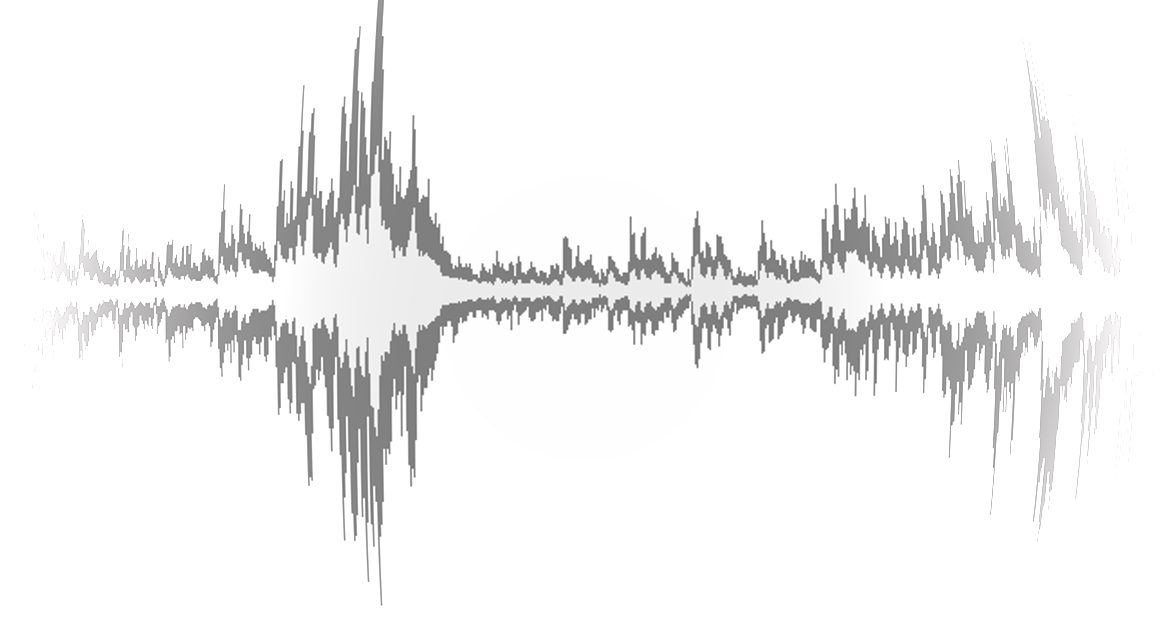
\includegraphics[width=\textwidth,height=3cm]{title}}


\begin{frame}
    \titlepage
    %\vspace{-5mm}
    \begin{flushright}
        \href{http://www.gtcmt.gatech.edu}{
\includegraphics[height=.8cm,keepaspectratio]{../shared/Logo_GTCMT_black}}
    \end{flushright}
\end{frame}


\section[intro]{introduction}
        \begin{frame}{Fourier transform}{overview}
            \begin{enumerate}
                \item   Fourier series to Fourier transform
                \item   properties of the Fourier transform
                \item   windowed Fourier transform (STFT)
                \item   transform of sampled time signals
                \item   Discrete Fourier Transform (DFT)
            \end{enumerate}
        \end{frame}

	\begin{frame}{Fourier transform}{introduction}
		%\vspace{-4mm}
        \begin{columns}
        \column{.4\linewidth}
		Fourier series is cool, but:
		\begin{itemize}
			\item	works only for periodic signals 
			\item	difficult to use for real-world analysis as it requires knowledge of fundamental frequency
			\item<2->[$\Rightarrow$]	\textbf{Fourier transform}
		\end{itemize}
        \column{.4\linewidth}
        \only<2->{
        \figwithmatlab{FourierTransform}
        }
        \end{columns}
	\end{frame}	
    \section{FS to FT}
	\begin{frame}{Fourier transform}{Fourier series revisited}
			\begin {equation*}
				c_k = \frac{1}{T_0}\int\limits_{-\nicefrac{T_0}{2}}^{\nicefrac{T_0}{2}} x(t) \e^{-\jom_0kt}\, dt \nonumber
			\end {equation*}
        \only<1-4>{    
        \begin{itemize}
            \item   Fourier series coefficients can be interpreted as \textbf{correlation coefficient} between signal and sinusoidals of different frequencies
            \item   only frequencies $k\omega_0$ are used
            ($\omega_0$ \textit{has to be known})
            \pause
            \item[$\Rightarrow$] Fourier series produces a \textbf{'line spectrum'}
            \bigskip
            \pause
            \item   distance between frequency components decreases as $T_0$ increases
            \pause
            \item[$\Rightarrow$]   aperiodic functions could be analyzed by increasing $T_0\rightarrow\infty$
        \end{itemize}
        }
        \only<5->{
        \begin{eqnarray*}
            &T_0 \rightarrow \infty&\\
            \pause
            \Rightarrow & k\omega_0 \rightarrow \omega\\
            \Rightarrow & \frac{1}{T_0} \rightarrow 0
        \end{eqnarray*}
        \pause
        \begin{itemize}
            \item[]   to avoid Zero result, multiply with $T_0$
        \end{itemize}
        }
        
        
        \vspace{70mm}
	\end{frame}	

\section{continuous FT}

	\begin{frame}{Fourier transform}{definition (continuous)}
        \begin{block}{Fourier transform definition}
		\begin {equation*}\label{eq:Fourier_transformation}
			X(\jom) = \mathfrak{F}[x(t)] = \int\limits_{-\infty}^{\infty} {x(t) \e^{-\jom t}\, dt}
		\end {equation*}
        \end{block}
	\end{frame}	

	\begin{frame}{Fourier transform}{example 1: rect window}
        \vspace{-8mm}
        \begin{footnotesize}
        \begin{eqnarray*}
            w_{\mathrm{R}}(t)	&=& \left\lbrace  
                        \begin{array}{ll} 
                                                    1, & -\frac{1}{2} \leq t \leq \frac{1}{2}\\ 
                          \vphantom{\frac{1}{1}} 	0, & \text{otherwise} \\ 
                        \end{array} 
                        \right. .
        \end{eqnarray*}
\pause
        \begin{eqnarray*}
            W_{\mathrm{R}}(\jom) 	&=& \int\limits_{-\infty}^{\infty} {w_{\mathrm{R}}(t)\e^{-\jom t}\,dt}\nonumber\\
                        &=& \int\limits_{-\nicefrac{1}{2}}^{\nicefrac{1}{2}} {\e^{-\jom t}\,dt}\nonumber\\
                        &=& \frac{1}{-\jom} \underbrace{\left(\e^{-\mathrm{j}\nicefrac{\omega}{2}}-\e^{\mathrm{j}\nicefrac{\omega}{2}}\right)}_{= -2j\sin\left(\nicefrac{\omega}{2}\right)}\nonumber\\
                        &=& \frac{\sin\left(\nicefrac{\omega}{2}\right)}{\nicefrac{\omega}{2}} = \si\left(\frac{\omega}{2}\right) .
        \end{eqnarray*}
        \end{footnotesize}
        \pause
        
        How will this change for different widths of $w_R$?
	\end{frame}	

	\begin{frame}{Fourier transform}{example 2: dirac}
        \vspace{-5mm}
        \begin{eqnarray*} % is this a proper definition??????
            \int\limits_{-\infty}^{\infty} \delta(t)\, dt &=& 1\label{eq:dirac_int} ,\\
            \delta(t) &=& 0\; \text{for all } t\neq 0 .
        \end{eqnarray*}
        \pause
        \begin{equation*}
            \Rightarrow \Delta(\jom) = \int\limits_{-\infty}^\infty \delta(t)e^{-\jom t}dt = e^{-\jom \cdot 0} = 1
        \end{equation*}
        \pause
        
        \bigskip
        shifted dirac: $\delta(t-\tau_0)$
         \begin{equation*}
            \Rightarrow \Delta(\jom) = \int\limits_{-\infty}^\infty \delta(t-\tau_0)e^{-\jom t}dt = e^{-\jom \tau_0}
        \end{equation*}
   \end{frame}	

\section{FT properties}
	\begin{frame}{Fourier transform}{property 1: invertibility}
		\begin{eqnarray*}\label{eq:ift}
			x(t) &=& \mathfrak{F}^{-1}[X(\jom)]\nonumber\\
			 &=& \frac{1}{2\pi}\int\limits_{-\infty}^{\infty} X(\jom) \e^{\jom t}\, d\omega 
		\end{eqnarray*}
        \bigskip
 
        \begin{itemize}
            \begin{footnotesize}
            \item[] reminder: signal reconstruction with Fourier series coefficients
                \begin {equation*}
                    x(t) = \sum\limits_{k=-\infty}^{\infty} c_k e^{\jom_0kt}
                \end {equation*}
            \end{footnotesize}
            \pause
            \item   \textbf{comments}:
                \begin{itemize}
                    \item   invertibility: no information is lost during this process!
                    \item   FT and IFT are very similar, largely equivalent
                \end{itemize}
        \end{itemize}
        

	\end{frame}	

	\begin{frame}{Fourier transform}{property 2: superposition}
		\begin{eqnarray*}
			y(t) &=& c_1\cdot x_1(t) + c_2\cdot x_2(t)\nonumber\\
			\mapsto&&\nonumber\\
			Y(\jom) &=& c_1\cdot X_1(\jom) + c_2\cdot X_2(\jom)\nonumber
		\end{eqnarray*}
		\pause
		\begin{itemize}
			\item[]	derivation
					\begin{footnotesize}
						\begin{eqnarray*}
							Y(\jom) &=& \int\limits_{-\infty}^{\infty} {\big(c_1\cdot x_1(t) + c_2\cdot x_2(t)\big)\cdot \e^{-\jom t}\, dt}\nonumber\\
							\pause
							&=& c_1\cdot \int\limits_{-\infty}^{\infty} {x_1(t)  \e^{-\jom t}\, dt} + c_2\cdot \int\limits_{-\infty}^{\infty} {x_2(t) \e^{-\jom t}\, dt}\nonumber\\
							\pause
							&=& c_1\cdot X_1(\jom) + c_2\cdot X_2(\jom) 
						\end{eqnarray*}
					\end{footnotesize}
		\end{itemize}
	\end{frame}	

	\begin{frame}{Fourier transform}{property 3: convolution and multiplication}
		\vspace{-7mm}
        \begin{eqnarray*}
			y(t) &= \int_{-\infty}^{\infty} {h(\tau) \cdot x(t-\tau)\, d\tau}\pause\mapsto 
			Y(\jom) &= H(\jom)\cdot X(\jom) \nonumber
		\end{eqnarray*}
		\pause
        \begin{columns}
        \column{.3\linewidth}
            derivation
        \column{.7\linewidth}
        \vspace{-5mm}
					\begin{footnotesize}
				\begin{eqnarray*}
					Y(\jom)	&=& \int_{-\infty}^{\infty} {y(t) \e^{-\jom t}\, dt}\nonumber\\
							\pause
								&=& \int_{-\infty}^{\infty} {\left(\int_{-\infty}^{\infty} {h(\tau) \cdot x(t-\tau)\, d\tau}\right) \e^{-\jom t}\, dt}\nonumber\\
							\pause
								&=& \int_{-\infty}^{\infty} {h(\tau) \int_{-\infty}^{\infty} {x(t-\tau)} \e^{-\jom t}\, dt\, d\tau}\nonumber\\
							\pause
								&=& \int_{-\infty}^{\infty} {h(\tau)  \e^{-\jom \tau} \underbrace{\int_{-\infty}^{\infty} {x(t-\tau)} \e^{-\jom (t-\tau)}\, d(t-\tau)}_{X(\jom)}\, d\tau}\nonumber\\
							\pause
								&=& \int_{-\infty}^{\infty} {h(\tau) \e^{-\jom \tau}\, d\tau} \cdot X(\jom)\nonumber\\
							\pause
								&=& H(\jom) \cdot X(\jom)\label{eq:mult_conv} 
				\end{eqnarray*}
					\end{footnotesize}
        \end{columns}
		%\begin{itemize}
			%\item[]	derivation
					%\begin{footnotesize}
				%\begin{eqnarray*}
					%Y(\jom)	&=& \int_{-\infty}^{\infty} {y(t) \e^{-\jom t}\, dt}\nonumber\\
							%\pause
								%&=& \int_{-\infty}^{\infty} {\left(\int_{-\infty}^{\infty} {h(\tau) \cdot x(t-\tau)\, d\tau}\right) \e^{-\jom t}\, dt}\nonumber\\
							%\pause
								%&=& \int_{-\infty}^{\infty} {h(\tau) \int_{-\infty}^{\infty} {x(t-\tau)} \e^{-\jom t}\, dt\, d\tau}\nonumber\\
							%\pause
								%&=& \int_{-\infty}^{\infty} {h(\tau)  \e^{-\jom \tau} \underbrace{\int_{-\infty}^{\infty} {x(t-\tau)} \e^{-\jom (t-\tau)}\, d(t-\tau)}_{X(\jom)}\, d\tau}\nonumber\\
							%\pause
								%&=& \int_{-\infty}^{\infty} {h(\tau) \e^{-\jom \tau}\, d\tau} \cdot X(\jom)\nonumber\\
							%\pause
								%&=& H(\jom) \cdot X(\jom)\label{eq:mult_conv} 
				%\end{eqnarray*}
					%\end{footnotesize}
		%\end{itemize}
	\end{frame}	

	\begin{frame}{Fourier transform}{property 4: Parseval's theorem}
		\begin{equation*}
			\int_{-\infty}^{\infty}{x^2(t)\, dt} = \frac{1}{2\pi}\int_{-\infty}^{\infty} {\left|X(\jom)\right|^2\, d\omega} 
		\end{equation*}
		\pause
		\begin{itemize}
			\item[]	derivation
			\begin{footnotesize}
				\begin{equation*}
					\int_{-\infty}^{\infty}{h(\tau)\cdot x(t-\tau)\, d\tau} = \frac{1}{2\pi}\int_{-\infty}^{\infty} {H(\jom)\cdot X(\jom) \e^{\jom t} d\omega}\nonumber
				\end{equation*}
				 \centering $H(\jom) \longrightarrow X^\ast (\jom)$ and $h(\tau)\longrightarrow x(-\tau)$, $t = 0$
							\pause
				\begin{eqnarray*}
					\int_{-\infty}^{\infty}{x(-\tau)\cdot x(-\tau)\, d\tau} &=& \frac{1}{2\pi}\int_{-\infty}^{\infty} {X^\ast (\jom)\cdot X(\jom) \, d\omega}\nonumber\\
					\pause
					\int_{-\infty}^{\infty}{x^2(t)\, dt} &=& \frac{1}{2\pi}\int_{-\infty}^{\infty} {\left|X(\jom)\right|^2\, d\omega} \nonumber
				\end{eqnarray*}
			\end{footnotesize}
		\end{itemize}
	\end{frame}	

	\begin{frame}{Fourier transform}{property 5: time \& frequency shift}
		\begin{equation*}\label{eq:fft_timeshift}
			y(t) = x(t-t_0)\rightarrow Y(\jom) = X(\jom)\e^{-\jom t_0} 
		\end{equation*} 
		\pause
		\begin{itemize}
			\item[]	derivation
			\begin{footnotesize}
				\begin{eqnarray*}
					\int\limits_{-\infty}^{\infty} {x(t-t_0) \e^{-\jom t}\, dt} &=& \int\limits_{-\infty}^{\infty} {x(\tau) \e^{-\jom (\tau + t_0)}\, d\tau}\nonumber\\
					\pause
					&=& \e^{-\jom t_0}\int\limits_{-\infty}^{\infty} {x(\tau) \e^{-\jom \tau}\, d\tau}\nonumber\\
					\pause
					&=& \e^{-\jom t_0} \cdot X(\jom) \nonumber
				\end{eqnarray*}
			\end{footnotesize}
		\end{itemize}
		\pause
		frequency shift:
		\begin{equation*}
					\frac{1}{2\pi}\int\limits_{-\infty}^{\infty} X(\mathrm{j}(\omega-\omega_0)) \e^{\jom t}\, d\omega = \e^{\jom_0 t}\cdot x(t) 		
		\end{equation*} 

	\end{frame}	

	\begin{frame}{Fourier transform}{property 6: symmetry 1/2}
		\begin{eqnarray*}
			|X(\jom)| &=& |X(-\jom)|\\
			\Phi_\mathrm{X}(\omega) &=& -\Phi_\mathrm{X}(-\omega) 
		\end{eqnarray*}

		\vspace{-5mm}
		\begin{itemize}
			\item<2->[]	derivation
			
			\begin{footnotesize}
				time signal sum of even and odd component $x_e(t), x_o(t)$:
				\begin{equation*}
					x(t) = \underbrace{\frac{1}{2}(x(t) + x(-t))}_{x_e(t)} + \underbrace{\frac{1}{2}(x(t) - x(-t))}_{x_o(t)} 
				\end{equation*}
				\pause
				\begin{equation*}
					X_e(\jom) = \int\limits_{-\infty}^{\infty}{x_e(t)\cos(\omega t)\,dt} - \mathrm{j} \underbrace{\int\limits_{-\infty}^{\infty}{x_e(t)\sin(\omega t)\,dt}}_{= 0}\nonumber
				\end{equation*}
				
		\vspace{-5mm}
				\begin{itemize}
					\item<4->[$\Rightarrow$]	$X_e(\jom)$ is real
					\item<4->[$\Rightarrow$]	$X_e(\jom) = X_e(-\jom)$ (substitute $x(t)$ with $x(-t)$)
				\end{itemize}
			\end{footnotesize}
		\end{itemize}
	\end{frame}	

	\begin{frame}{Fourier transform}{property 6: symmetry 2/2}
		\begin{eqnarray*}
			|X(\jom)| &=& |X(-\jom)|\\
			\Phi_\mathrm{X}(\omega) &=& -\Phi_\mathrm{X}(-\omega) 
		\end{eqnarray*}
		\pause
		\vspace{-5mm}
		\begin{itemize}
			\item[]	derivation
			
			\begin{footnotesize}
				time signal sum of even and odd component $x_e(t), x_o(t)$:
				\begin{equation*}
					x(t) = \underbrace{\frac{1}{2}(x(t) + x(-t))}_{x_e(t)} + \underbrace{\frac{1}{2}(x(t) - x(-t))}_{x_o(t)} 
				\end{equation*}
				\pause
				\begin{equation*}
					X_o(\jom) = \underbrace{\int\limits_{-\infty}^{\infty}{x_o(t)\cos(\omega t)\,dt}}_{=0} - \mathrm{j} \int\limits_{-\infty}^{\infty}{x_o(t)\sin(\omega t)\,dt} \nonumber
				\end{equation*}
				\pause
		\vspace{-5mm}
				\begin{itemize}
					\item[$\Rightarrow$]	$X_o(\jom)$ is imaginary
					\item[$\Rightarrow$]	$X_o(\jom) = -X_o(-\jom)$ (substitute $x(t)$ with $-x(-t)$)
				\end{itemize}
			\end{footnotesize}
		\end{itemize}
	\end{frame}	

	\begin{frame}{Fourier transform}{property 7: time \& frequency scaling}
				\begin{equation*}
					y(t) = x(c\cdot t) \mapsto Y(\jom) = \frac{1}{|c|}X\left(j\frac{\omega}{c}\right) 
				\end{equation*}
		\pause
		\begin{itemize}
			\item[]	derivation (positive c)
			\begin{footnotesize}
				\begin{eqnarray*}
					Y(\jom) &=& \int\limits_{-\infty}^{\infty} {x(c\cdot t) \e^{-\jom t}\, dt}\nonumber\\
					\pause
					&=& \int\limits_{-\infty}^{\infty} {x(\tau) \e^{-\jom \frac{\tau}{c}}\, d\frac{\tau}{c}}\nonumber\\
					\pause
					&=& \frac{1}{c}\int\limits_{-\infty}^{\infty} {x(\tau) \e^{-\mathrm{j} \frac{\omega}{c} \tau}\, d\tau}\nonumber\\
					\pause
					&=& \frac{1}{c} X\left(\mathrm{j}\frac{\omega}{c}\right) \nonumber
				\end{eqnarray*}
			\end{footnotesize}
		\end{itemize}
	\end{frame}	

	\begin{frame}{Fourier transform}{examples}
			\question{What is the FT of}
			\begin{itemize}
				\item	delta function
				\item	constant
				\item	cosine
				\item	rectangular window
				\item	delta pulse
			\end{itemize}
	\end{frame}	


\section{STFT}
	\begin{frame}{Fourier transform}{STFT introduction}
		short time Fourier transform (STFT):\linebreak compute Fourier transform only over a segment

		\vspace{3mm}		
		\pause
		reasons:
		\begin{itemize}
			\item	\textbf{signal properties}: choose quasi-periodic segment
			\item	\textbf{perception}: ear analyzes short segments of signal
			\item	\textbf{hardware}: Fourier transform is inefficient and memory consuming for very long input segments
		\end{itemize}
		\pause
        \bigskip
		$\Rightarrow$ multiply a \textbf{window} with the signal
	\end{frame}	

	\begin{frame}{Fourier transform}{STFT: windowing}
        \includeanimation{Windowing}{01}{05}{1}
        %\begin{center}
            %\animategraphics[scale=.8]        
        %\end{center}
	\end{frame}	
    
	\begin{frame}{Fourier transform}{reminder: FT of rectangular window}
        \vspace{-8mm}
        \begin{footnotesize}
        \begin{eqnarray*}
            w_{\mathrm{R}}(t)	&=& \left\lbrace  
                        \begin{array}{ll} 
                                                    1, & -L \leq t \leq L\\ 
                          \vphantom{\frac{1}{1}} 	0, & \text{otherwise} \\ 
                        \end{array} 
                        \right. .
        \end{eqnarray*}
\pause
        \begin{eqnarray*}
            W_{\mathrm{R}}(\jom) 	&=& \int\limits_{-\infty}^{\infty} {w_{\mathrm{R}}(t)\e^{-\jom t}\,dt}\nonumber\\
                        &=& \int\limits_{-L}^{L} {\e^{-\jom t}\,dt}\nonumber\\
                        &=& \frac{1}{-\jom} \underbrace{\left(\e^{-\mathrm{j}{\omega L}}-\e^{\mathrm{j}{\omega L}}\right)}_{= -2j\sin\left({L\omega}\right)}\nonumber\\
                        &=& \frac{2\sin\left({L\omega}\right)}{{\omega}}  .
        \end{eqnarray*}
        \end{footnotesize}
	\end{frame}	

	\begin{frame}{Fourier transform}{question: FT of triangular window}
        \question{Given your knowledge of the frequency transform of the rect window and both the FT \& LTI system properties, what is the FT of a triangular window}
        \bigskip
        \bigskip
        \begin{enumerate}
            \item   triangular window is output convolution of two rectangular windows
            \item   convolution in time domain is multiplication in the frequency domain
            \item[$\Rightarrow$] sinc squared
        \end{enumerate}
	\end{frame}	

	\begin{frame}{Fourier transform}{STFT: window functions}
		multiplication in time domain $\rightarrow$ convolution in frequency domain
        \begin{equation*}
            x_\mathrm{W}(t) = x(t)\cdot w(t) \rightarrow X_\mathrm{W}(\jom) = X(\jom) \ast W(\jom)
        \end{equation*}

		\pause		
		$\Rightarrow$\textbf{spectral leakage}
        \figwithmatlab{SpectralWindows}
		%\begin{figure}
			%\centering
				%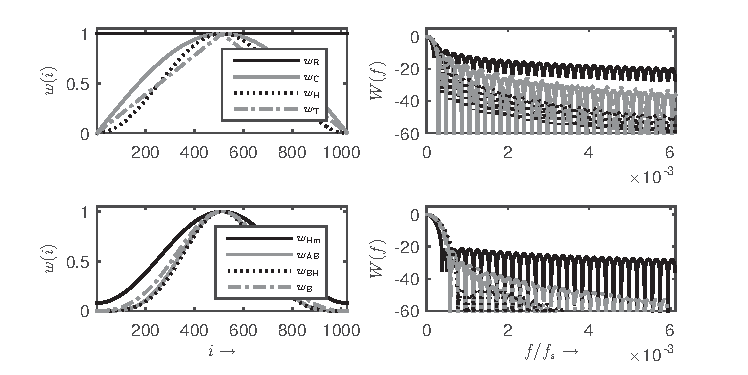
\includegraphics[scale=.8]{windows.pdf}
			%\label{fig:windows}
		%\end{figure}
	\end{frame}	

	\begin{frame}{Fourier transform}{STFT: window function properties}
		\begin{itemize}
			\item	\textbf{main lobe width}
                \begin{itemize}
                    \item   how much does the main lobe ``smear'' a peak
                \end{itemize}
            \bigskip
			\item<2->	\textbf{side lobe height}
                \begin{itemize}
                    \item   how dominant is the (highest) side lobe
                \end{itemize}
			\bigskip
            \item<3->	\textbf{side lobe attenuation/fall-off}
                \begin{itemize}
                    \item   how much influence have distant sidelobes
                \end{itemize}
            \bigskip
            \item<4->\textbf{process and scalloping loss} (DFT)
                \begin{itemize}
                    \item   how accurate is the amplitude (best case and worst case)
                \end{itemize}
		\end{itemize}
	\end{frame}	

	\begin{frame}{Fourier transform}{STFT: typical window functions}
        \begin{itemize}
            \item   (rectangular window) $w_\mathrm{R}(t)$
            \smallskip
            \item   \textbf{von-Hann window}: $w_\mathrm{H}(t) = w_\mathrm{R}(t)\cdot\nicefrac{1}{2}\left(1 + \cos\left(\frac{\pi}{2}t\right) \right)$
            \smallskip
            \item   \textbf{Hamming window}: $w_\mathrm{Hm}(t) = w_\mathrm{R}(t)\cdot\nicefrac{25}{46} + \nicefrac{42}{46}\cos\left(\frac{\pi}{2}t\right)$
            \smallskip
            \item   \textbf{Cosine window}: $w_\mathrm{C}(t) = w_\mathrm{R}(t)\cdot\cos\left(\frac{\pi}{2}t\right)$
            \smallskip
            \item   \textbf{Blackman-Harris window}:
                    \begin{equation*}
						w_\mathrm{BH}(t) = w_{\mathrm{R}}(t)\sum\limits_{m=0}^{3}{b_m\cos\left(\frac{\pi}{2}mt\right)} .
					\end{equation*}
                    with $b_0 = 0.35875,\, b_1 = 0.48829,\, b_2 = 0.14128, b_3 = 0.01168$
        \end{itemize}
	\end{frame}	

\section{FT of sampled input}
	\begin{frame}{Fourier transform}{sampled time signals 1/2}
		\vspace{-5mm}
        \begin{eqnarray*}\label{eq:ft_sampled}
			\mathfrak{F}[x(i)] 	&=& \mathfrak{F}[x(t)\cdot \delta_\mathrm{T}(t)]\nonumber\\
			\pause
								&=& \mathfrak{F}[x(t)]\ast \mathfrak{F}[\delta_\mathrm{T}(t)]\nonumber\\
								&=& X(\jom)\ast \Delta_\mathrm{T}(\jom) \nonumber
		\end{eqnarray*}
        \only<3>{
            \vspace{-5mm}
            \figwithmatlab{SpecSampling}
        }
		\only<4>{
        \begin{columns}
        \column{.3\linewidth}
        %\visible<4->{
		transformed signal is 
        \begin{itemize}
            \item   still \textbf{continuous}
            \item   \textbf{periodic}
        \end{itemize}
        %}
        \column{.7\linewidth}
        \includeanimation{Aliasing}{01}{48}{10}
        \end{columns}
        }
	\end{frame}	
	\begin{frame}{Fourier transform}{sampled time signals 2/2}
        \begin{eqnarray*}
            X(\jOm) &=& \sum\limits_{i=-\infty}^{\infty} x(i)e^{-\jOm i}\\
            x(i) &=& \frac{1}{2\pi}\int\limits_{-\pi}^{\pi}X(\jOm)e^{\jOm i} d\Omega\\
            \Omega &=& 2\pi\frac{\omega}{\omega_T}
        \end{eqnarray*}
	\end{frame}	


\section{DFT}
	\begin{frame}{Fourier transform}{DFT}
		digital domain: requires discrete frequency values:
		
		$\Rightarrow$ \textbf{Discrete Fourier transform (DFT)}
		\begin{equation*}
			X(k) = \sum\limits_{i=0}^{\mathcal{K}-1}{x(i)\e^{-\mathrm{j}ki\frac{2\pi}{\mathcal{K}}}}
		\end{equation*}
        \pause
        alternative notation
		\begin{equation*}
			X(k\Omega_\mathcal{K}) = \sum\limits_{i=0}^{\mathcal{K}-1}{x(i)\e^{-\mathrm{j}ki\Omega_\mathcal{K}}}
		\end{equation*}
		
		\pause
        \bigskip
		2 interpretations:
		\begin{itemize}
			\item	sampled continuous Fourier transform
			\item	continuous Fourier transform of periodically extended time domain segment
		\end{itemize}
	\end{frame}	

	\begin{frame}{Fourier transform}{DFT frequency resolution}
        \begin{itemize}
            \item   DFT frequency resolution depends on 
                \begin{itemize}
                    \item   block length $\mathcal{K}$
                    \item   sample rate $\omega_T$ (spectrum is periodic with $\omega_T$)
                \end{itemize}
            \pause
            \item   $\Rightarrow \Delta\omega = \frac{\omega_T}{\mathcal{K}}$
            \pause
            \bigskip
            \item   increasing the DFT length increases frequency resolution
                \begin{itemize}
                    \item   decreasing time resolution
                    \item   zero-padding
                \end{itemize}
        \end{itemize}
	\end{frame}	
	%\begin{frame}{Fourier transform}{best case vs worst case}
		%\begin{figure}
			%\centering
				%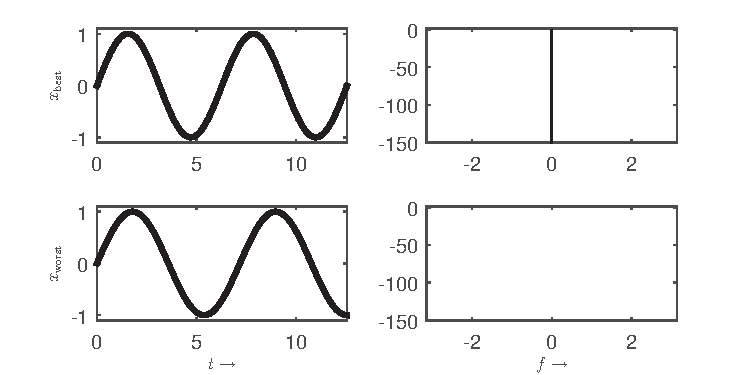
\includegraphics[scale=.7]{graph/bestworstcase}
		%\end{figure}
	%\end{frame}	

	\begin{frame}{Fourier transform}{DFT vs FFT}
        \begin{itemize}
            \item   FFT is an algorithm to efficiently calculate the DFT
            \item   result is \textbf{identical}
            \item   efficiency:
                \begin{itemize}
                    \item   DFT: $\mathcal{K}^2$ complex multiplications
                    \item   FFT: $\nicefrac{\mathcal{K}}{2}\log_2(\mathcal{K})$ complex multiplications
                \end{itemize}
        \end{itemize}
        
        \begin{table}
            \centering
                \begin{tabular}{l|ccc}
                    $\mathcal{K}$  & DFT mult & FFT mult & efficiency\\ \hline
                    
                    $256$ & $2^{16}$ & $1024$ & $64:1$\\
                    $512$ & $2^{18}$ & $2304$ & $114:1$\\
                    $1024$ & $2^{20}$ & $5120$ & $205:1$\\
                    $2048$ & $2^{22}$ & $11264$ & $372:1$\\
                    $4096$ & $2^{24}$ & $24576$ & $683:1$\\
                \end{tabular}
        \end{table}
	\end{frame}	

	\begin{frame}{Fourier transform}{STFT: spectrogram}
           \vspace{-2mm}
            \begin{itemize}
                \item   spectrogram allows to visualize temporal changes in the spectrum
                \item   displays the \textit{magnitude spectrum }only
            \end{itemize}
            \vspace{-8mm}
            \begin{columns}
                \column{.9\linewidth}
                    \figwithmatlab{Specgram}
                \column{.1\linewidth}
                    \begin{figure}
                    \includeaudio{sax_example}
                    \end{figure}
            \end{columns}
	\end{frame}	

    \section[summary]{summary}
            \begin{frame}{Fourier transform}{summary 1/2}
                \textbf{FT properties}
                \begin{enumerate}
                    \item   invertibility
                    \item   linearity
                    \item   convolution --- multiplication
                    \item   Parseval's theorem
                    \item   time shift --- phase shift
                    \item   symmetry
                    \item   time scaling --- frequency scaling
                \end{enumerate}
            \end{frame}	
    
            \begin{frame}{Fourier transform}{summary 2/2}
                \begin{enumerate}
                    \item   Fourier series can describe any periodic function $\rightarrow$ discrete ``spectrum''
                    \item   continuous FT transforms any continuous function $\rightarrow$ continuous spectrum
                    \item   STFT transforms a segment of the signal $\rightarrow$ convolution with window spectrum
                    \item   FT of sampled signals $\rightarrow$ periodic
                    \item   DFT $\rightarrow$ sampled FT of periodic continuation
                \end{enumerate}
                    \pause
                \begin{itemize}
                    \item   \textbf{spectrum is periodic $\leftrightarrow$ time signal is discrete}
                    \item   \textbf{spectrum is discrete $\leftrightarrow$ time signal is periodic}
                \end{itemize}
            \end{frame}	
    
\end{document}

